\documentclass{article}
\usepackage{tikz}
\usetikzlibrary{positioning} % enables relative placement

\begin{document}

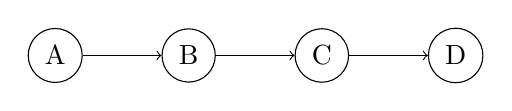
\begin{tikzpicture}[nodes={draw,circle}]
  % --- Nodes placed relative to each other ---
  \node (A) {A};
  \node (B) [right=of A] {B};
  \node (C) [right=of B] {C};
  \node (D) [right=of C] {D};

  % --- Path edges ---
  \draw[->] (A) -- (B);
  \draw[->] (B) -- (C);
  \draw[->] (C) -- (D);
\end{tikzpicture}

\end{document}
